\begin{frame}
    \frametitle{\problemtitle}

    \begin{itemize}
        \item Determine the minimum number of \emph{robberies} to make a binary
            tree \emph{strongly balanced}.
        \item A robbery is to take a leaf and remove it, and doing so may turn its parent vertex into a leaf.
        \item A tree is strongly balanced when for each vertex the height of its
            left and right subtree differs by at most $1$.
        \item The tree has $1 \leq n \leq 2 \cdot 10^5$ vertices.
    \end{itemize}

    \vspace{0.5em}

    \centering
    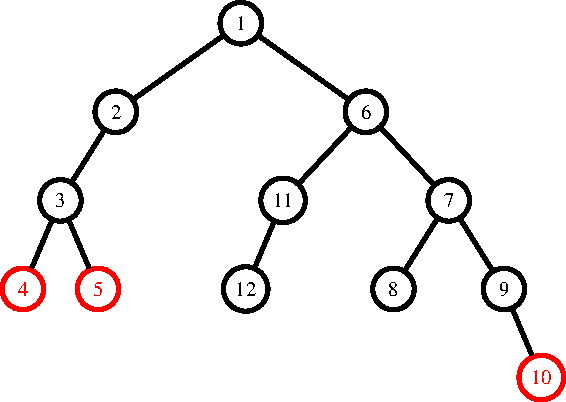
\includegraphics[height=0.4\textheight]{sample}

    \small
    Illustration of Sample Input 2.
    The tree becomes strongly balanced after removing the three vertices marked in red ($4$, $5$, and $10$);
    the minimum number of vertices that need to be removed to make the tree strongly balanced.
\end{frame}
